\section{Fahrcontroller}

\begin{frame}
	\frametitle{Anpassungen}	
	\begin{columns}
		\begin{column}{0.6 \textwidth}
			\begin{itemize}
				\item Studienarbeit als Basis
				\item Interface auf Mainboard
				\item Kommunikation
				\item Rest bei Gleitkommaoperationen
				\item Kalibrierung
			\end{itemize}
		\end{column}
		\begin{column}{0.4 \textwidth}
			\vspace{-2.8em}
			\begin{figure}[h]
				\centering
				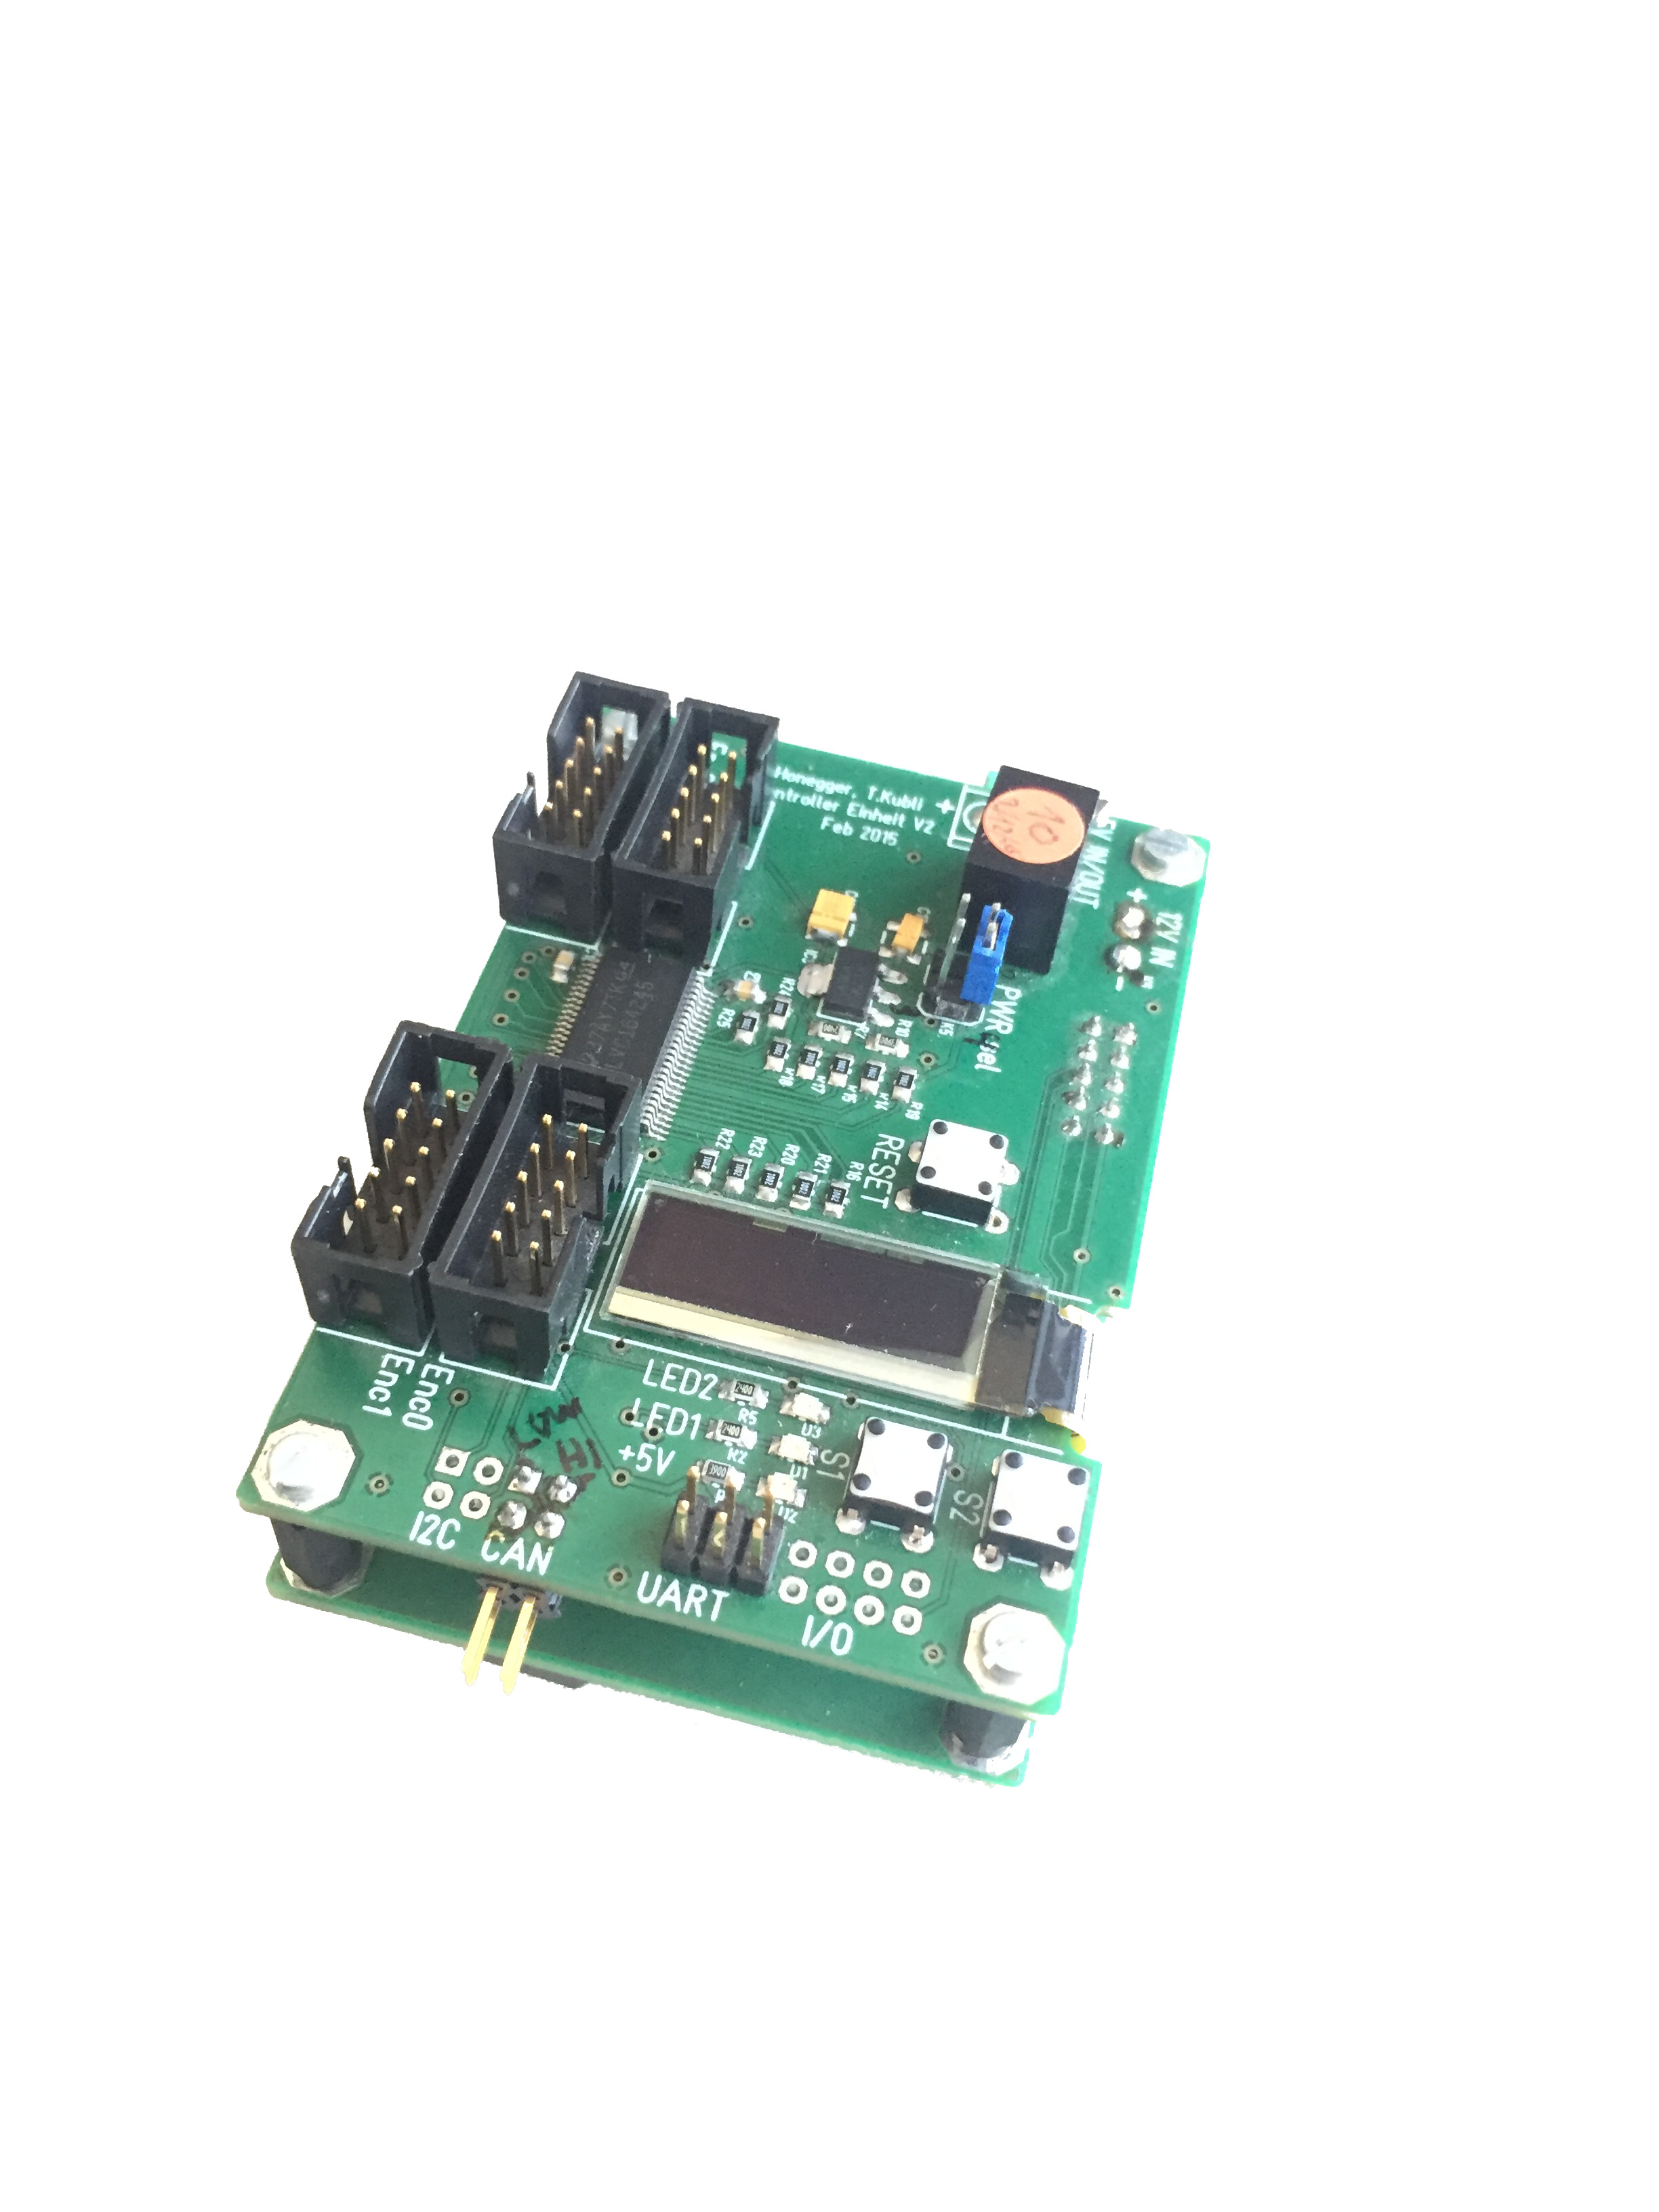
\includegraphics[width = 1 \textwidth]{../images/presentation/dc.jpg}
			\end{figure}
		\end{column}
	\end{columns}
	

\end{frame}

\begin{frame}
	\frametitle{Kalibrieren}
	\begin{itemize}
		\item verbesserte Fehlerberechnung
		\item Bedienung über Display
		\item Konfigurationsdaten auf USB-Stick
		\item getrennte Kalibrierung für Vorwärts- und Rückwärtsfahrt
	\end{itemize}
\end{frame}

\begin{frame}
	\frametitle{Probleme}
	\begin{itemize}
		\item Synchronisation schwierig
		\item kein vorausschauendes Fahren
		\item ungenaues Fahren
		\item Reglereinstellung mühsam
	\end{itemize}
\end{frame}